\documentclass[12pt,dvipdfmx]{beamer}
\usepackage{graphicx}
\DeclareGraphicsExtensions{.pdf}
\DeclareGraphicsExtensions{.eps}
\graphicspath{{out/tex/svg/}{out/tex/lsvg/}}
\usepackage{listings}
\usepackage{fancybox}
\usepackage{hyperref}
\usepackage{color}

\newcommand{\plusequal}{\mbox{\tt\ += }}
\newcommand{\minusequal}{\mbox{\tt\ -= }}
\newcommand{\divequal}{\mbox{\tt\ /= }}
\newcommand{\plusplus}{\mbox{\tt\ ++ }}

%%%%%%%%%%%%%%%%%%%%%%%%%%%
%%% themes
%%%%%%%%%%%%%%%%%%%%%%%%%%%
%\usetheme{Szeged} 
\usetheme{Madrid}

%% no navigation bar
% default boxes Bergen Boadilla Madrid Pittsburgh Rochester
%% tree-like navigation bar
% Antibes JuanLesPins Montpellier
%% toc sidebar
% Berkeley PaloAlto Goettingen Marburg Hannover Berlin Ilmenau Dresden Darmstadt Frankfurt Singapore Szeged
%% Section and Subsection Tables
% Copenhagen Luebeck Malmoe Warsaw

%%%%%%%%%%%%%%%%%%%%%%%%%%%
%%% innerthemes
%%%%%%%%%%%%%%%%%%%%%%%%%%%
% \useinnertheme{circles}       % default circles rectangles rounded inmargin

%%%%%%%%%%%%%%%%%%%%%%%%%%%
%%% outerthemes
%%%%%%%%%%%%%%%%%%%%%%%%%%%
% outertheme
% \useoutertheme{default}       % default infolines miniframes smoothbars sidebar sprit shadow tree smoothtree


%%%%%%%%%%%%%%%%%%%%%%%%%%%
%%% colorthemes
%%%%%%%%%%%%%%%%%%%%%%%%%%%
\usecolortheme{seahorse}
%% special purpose
% default structure sidebartab 
%% complete 
% albatross beetle crane dove fly seagull 
%% inner
% lily orchid rose
%% outer
% whale seahorse dolphin

%%%%%%%%%%%%%%%%%%%%%%%%%%%
%%% fontthemes
%%%%%%%%%%%%%%%%%%%%%%%%%%%
\usefonttheme{serif}  
% default professionalfonts serif structurebold structureitalicserif structuresmallcapsserif

%%%%%%%%%%%%%%%%%%%%%%%%%%%
%%% generally useful beamer settings
%%%%%%%%%%%%%%%%%%%%%%%%%%%
% 
\AtBeginDvi{\special{pdf:tounicode EUC-UCS2}}
% do not show navigation
\setbeamertemplate{navigation symbols}{}
% show page numbers
\setbeamertemplate{footline}[frame number]


%%%%%%%%%%%%%%%%%%%%%%%%%%%
%%% define some colors for convenience
%%%%%%%%%%%%%%%%%%%%%%%%%%%

\newcommand{\mido}[1]{{\color{green}#1}}
\newcommand{\mura}[1]{{\color{purple}#1}}
\newcommand{\ore}[1]{{\color{orange}#1}}
\newcommand{\ao}[1]{{\color{blue}#1}}
\newcommand{\aka}[1]{{\color{red}#1}}

\setbeamercolor{ex}{bg=cyan!20!white}

%%%%%%%%%%%%%%%%%%%%%%%%%%%
%%% how to typset code
%%%%%%%%%%%%%%%%%%%%%%%%%%%

\lstset{language = C,
numbers = left,
numberstyle = {\tiny \emph},
numbersep = 10pt,
breaklines = true,
breakindent = 40pt,
frame = tlRB,
frameround = ffft,
framesep = 3pt,
rulesep = 1pt,
rulecolor = {\color{blue}},
rulesepcolor = {\color{blue}},
flexiblecolumns = true,
keepspaces = true,
basicstyle = \ttfamily\scriptsize,
identifierstyle = ,
commentstyle = \it\scriptsize,
stringstyle = ,
showstringspaces = false,
tabsize = 4,
escapechar=\@,
}

\title{SIMD Programming}
\institute{}
\author{Kenjiro Taura}
\date{}

\AtBeginSection[] % Do nothing for \section*
{
\begin{frame}
\frametitle{Contents}
\tableofcontents[currentsection,currentsubsection]
\end{frame}
}

\AtBeginSubsection[] % Do nothing for \section*
{
\begin{frame}
\frametitle{Contents}
\tableofcontents[currentsection,currentsubsection]
\end{frame}
}

\begin{document}
\maketitle

%%%%%%%%%%%%%%%%%%%%%%%%%%%%%%%%%% 
\begin{frame}
\frametitle{Contents}
\tableofcontents
\end{frame}

\iffalse
%%%%%%%%%%%%%%%%%%%%%%%%%%%%%%%%%% 
%%%%%%%%%%%%%%%%%%%%%%%%%%%%%%%%%% 
\section{Introduction}
%%%%%%%%%%%%%%%%%%%%%%%%%%%%%%%%%% 
%%%%%%%%%%%%%%%%%%%%%%%%%%%%%%%%%% 

%%%%%%%%%%%%%%%%% 
\begin{frame}[fragile]
\frametitle{Remember performance of matrix-matrix multiply?}

\begin{itemize}
\item []
\begin{lstlisting}
void gemm(long n, /* n = 2400 */
          float A[n][n], float B[n][n], float C[n][n]) {
  long i, j, k;
  for (i = 0; i < n; i++)
    for (j = 0; j < n; j++)
      for (k = 0; k < n; k++)
        C[i][j] += A[i][k] * B[k][j];
}
\end{lstlisting}

% \item<2-> []
% \begin{lstlisting}
% $ make
% gcc -O3 -o simple_mm mm.c
% gcc -O3 -DUSE_BLAS -o blas_mm mm.c -lopenblas
% \end{lstlisting} %$

\item []
\begin{lstlisting}
$ ./simple_mm 
C[1200][1200] = 3011.114014
 in 56.382360 sec
 @\ao{\texttt{2.451831 GFLOPS}}@
\end{lstlisting} %$

\item []
\begin{lstlisting}
$ ./opt_mm 
C[1200][1200] = 3011.108154
 in 1.302980 sec
 @\ao{\texttt{106.095263 GFLOPS}}@
\end{lstlisting} %$
\end{itemize}

\end{frame}

%%%%%%%%%%%%%%%%%%%%%%%%%%%%%%%%%% 
\begin{frame}
\frametitle{What is the theoretical limit?}
\begin{itemize}
\item Intel Skylake processor
\item its \ao{\it single core} can execute, in \ao{\it every cycle},
  \begin{itemize}
  \item two \ao{\it fused multiply-add instructions}
  \item and others (e.g., integer arithmetic, load, store, \ldots) 
    I'll cover later
  \end{itemize}
\item a single fused multiply-add \ao{\it instruction}
  can multiply/add \ao{\it eight} double-precision 
  or \ao{\it sixteen} single-precision operands
\item \ao{Single Instruction Multiple Data (SIMD)} instructions
\end{itemize}
\end{frame}

%%%%%%%%%%%%%%%%%%%%%%%%%%%%%%%%%% 
\begin{frame}
\frametitle{Terminology}
\begin{itemize}
\item \ao{flops:} floating point operations
\item \ao{FLOPS:} Floating Point Operations Per Second
\item Practically,
\begin{eqnarray*}
  &   & \mbox{Peak FLOPS of a machine} \\
  & = & 2 \\
  & \times & \mbox{vector width} \\
  & \times & \mbox{max FMA instructions per cycle (IPC)} \\
  & \times & \mbox{cycles per second (frequency)} \\
  & \times & \mbox{the number of cores} \\
\end{eqnarray*}
\end{itemize}
\end{frame}

%%%%%%%%%%%%%%%%%%%%%%%%%%%%%%%%%% 
\begin{frame}
\frametitle{Peak flops/cycle of recent cores}

\begin{itemize}
\item Recent processors increasingly rely on SIMD
  as an energy efficient way to boost peak FLOPS
\end{itemize}

\begin{center}
{\scriptsize
\begin{tabular}{|l|c|c|c|c|c|}\hline
Microarchitecture & ISA    & throughput    & vector   & max SP flops/cycle \\
                  &        & (per clock)   & width (SP) & /core          \\
\hline
Nehalem           & SSE     & 1 add + 1 mul & 4     & 8  \\
Sandy Bridge      & AVX     & 1 add + 1 mul & 8     & 16 \\
Haswell           & AVX2    & 2 fmas        & 8     & 32 \\
\ao{Skylake}      & AVX-512 & 2 fmas        & 16    & 64 \\
\ao{Knights Landing (Mill)} & AVX-512       & 2 fmas & 16    & 64 \\
\hline
\end{tabular}
}
\end{center}

\begin{itemize}
\item ISA : Instruction Set Architecture
\item register width : the number of \ao{\em single precision} operands 
\item fma : fused multiply-add instruction
\item e.g.,
  Peak FLOPS of a machine having 2 $\times$ Intel Xeon Gold 6130 (2.10GHz, 32 cores) $=$ 8.6 TFLOPS
\end{itemize}
\end{frame}

%%%%%%%%%%%%%%%%%%%%%%%%%%%%%%%%%% 
\begin{frame}
\frametitle{The goal}

\begin{itemize}
\item practical ways to use SIMD instructions
\item basics of processors to know
  what kind of code can get close-to-peak performance
\end{itemize}

\end{frame}
\fi

%%%%%%%%%%%%%%%%%%%%%%%%%%%%%%%%%% 
%%%%%%%%%%%%%%%%%%%%%%%%%%%%%%%%%% 
\section{SIMD Instructions}
%%%%%%%%%%%%%%%%%%%%%%%%%%%%%%%%%% 
%%%%%%%%%%%%%%%%%%%%%%%%%%%%%%%%%% 

%%%%%%%%%%%%%%%%%%%%%%%%%%%%%%%%%% 
\begin{frame}
  \frametitle{SIMD : basic concepts}
  \begin{itemize}
  \item \ao{SIMD} : single instruction multiple data
  \item a \ao{\it SIMD register} (or a \ao{\it vector register})
    can hold many values (2 - 16 values or more) of a single type
  \item a \ao{\it SIMD instruction} is an instruction that
    can apply (typically the same) operation on all or some values on a SIMD register(s)
  \item each value in a SIMD register is called a \ao{\it SIMD lane}
    or simply a \ao{\it lane}
  \item they are indispensable tools for CPUs to get performance
  \end{itemize}

  \begin{center}
    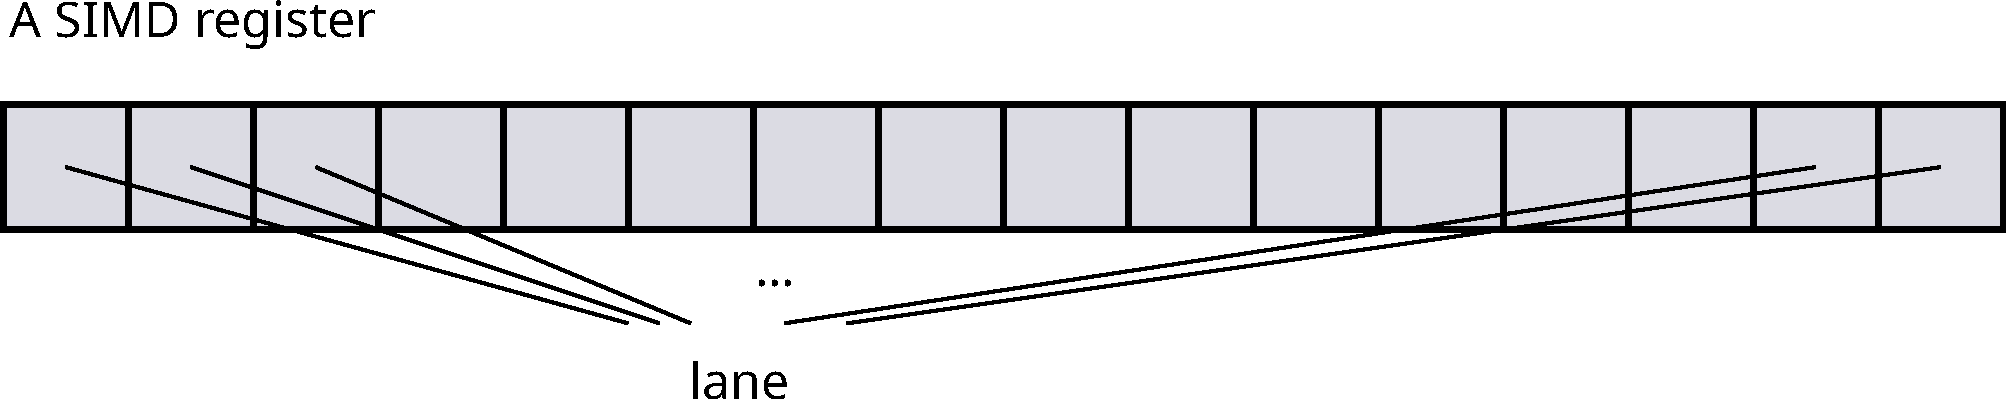
\includegraphics[width=0.7\textwidth]{out/pdf/svg/simd_registers_1.pdf}
  \end{center}
\end{frame}


%%%%%%%%%%%%%%%%%%%%%%%%%%%%%%%%%% 
\begin{frame}
\frametitle{Evolving Intel instruction set}

\begin{itemize}
\item Recent processors increasingly rely on SIMD
  as an energy efficient way to boost peak FLOPS
\end{itemize}

\begin{center}
{\scriptsize
\begin{tabular}{|l|c|c|c|c|c|}\hline
Microarchitecture & ISA    & vector        & throughput & max SP flops/cycle \\
                  &        & width (SP)    & (per clock)  & /core          \\
\hline
Nehalem           & SSE     & 4 & 1 add + 1 mul      & 8  \\
Sandy Bridge      & AVX     & 8 & 1 add + 1 mul     & 16 \\
Haswell           & AVX2    & 8 & 2 fmas             & 32 \\
\ao{Ice Lake}     & \ao{AVX-512} & \ao{16}  & \ao{2 fmas} & \ao{64} \\
\hline
\end{tabular}
}
\end{center}

\begin{itemize}
\item ISA : Instruction Set Architecture
\item vector width : the number of single precision (SP) operands 
\item fma : fused multiply-add instruction
\item e.g.,
  Peak FLOPS of a machine having 2 $\times$ Intel Xeon Gold 6130 (2.10GHz, 32 cores) $=$ 8.6 TFLOPS
\item no SIMD? $\rightarrow$ can tap {\it at most 1/16} of SP peak performance on machines having AVX-512
\end{itemize}
\end{frame}



%%%%%%%%%%%%%%%%%%%%%%%%%%%%%%%%%% 
\begin{frame}
\frametitle{Intel SIMD instructions at a glance}
Some example \ao{AVX-512F} (a subset of AVX-512) instructions
\begin{center}
{\footnotesize
\begin{tabular}{|l|l|l|}\hline
operation & syntax                         & C-like expression \\\hline
multiply & {\tt \ao{vmulps} \%zmm0,\%zmm1,\%zmm2} & {\tt zmm2 = zmm1 * zmm0} \\
add      & {\tt \ao{vaddps} \%zmm0,\%zmm1,\%zmm2} & {\tt zmm2 = zmm1 + zmm0} \\
fmadd    & {\tt \ao{vfmadd132ps} \%zmm0,\%zmm1,\%zmm2} & {\tt zmm2 = zmm0*zmm2+zmm1} \\
load     & {\tt \ao{vmovups} 256(\%rax),\%zmm0}   & {\tt zmm0 = *(rax+256)} \\
store    & {\tt \ao{vmovups} \%zmm0,256(\%rax)}   & {\tt *(rax+256) = zmm0} \\
\hline
\end{tabular}}
\end{center}

\begin{itemize}
\item {\tt zmm0} \ldots {\tt zmm31} are 512 bit registers; each can hold
  \begin{itemize}
  \item 16 single-precision ({\tt float} of C; 32 bits) or
  \item 8 double-precision ({\tt double} of C; 64 bits) 
  \item [] floating point numbers
  \end{itemize}
\item {\tt XXXps} stands for {\em \ao{p}acked \ao{s}ingle precision}
\end{itemize}
\end{frame}

%%%%%%%%%%%%%%%%%%%%%%%%%%%%%%%%%% 
\begin{frame}
  \frametitle{xmm, ymm and zmm registers}
  \begin{itemize}
  \item ISA and available registers
{\small
    \begin{tabular}{|l|c|}\hline
ISA     & registers         \\\hline
SSE     & {\tt xmm0, } \ldots {\tt xmm15}  \\
AVX     & \{{\tt x,y}\}{\tt mm0},  \ldots \{{\tt x,y}\}{\tt mm15} \\
AVX-512 & \{{\tt x,y,z}\}{\tt mm0}, \ldots \{{\tt x,y,z}\}{\tt mm31} \\\hline
\end{tabular}}
\item registers and their widths \ao{\it (vector widths)}
{\small
  \begin{tabular}{|l|r|}\hline
register names & register width (bits) \\\hline
xmm$i$   & 128    \\
ymm$i$   & 256    \\
zmm$i$   & 512    \\\hline
  \end{tabular}}

\item xmm$i$, ymm$i$ and zmm$i$ are \ao{\it aliased}

  \begin{center}
    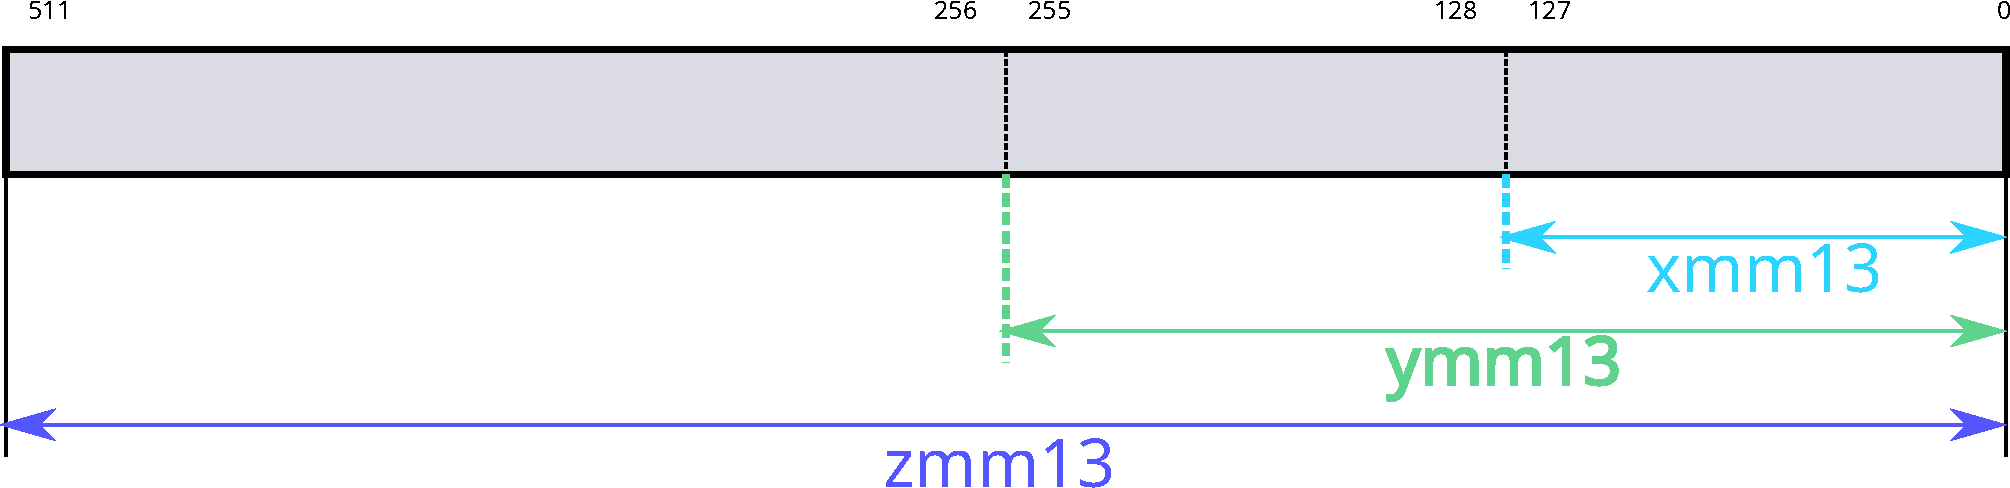
\includegraphics[width=0.7\textwidth]{out/pdf/svg/xmm_ymm_zmm_1.pdf}
  \end{center}
  
\end{itemize}  
\end{frame}


%%%%%%%%%%%%%%%%%%%%%%%%%%%%%%%%%% 
\begin{frame}
  \frametitle{Intel SIMD instructions at a glance}
  \begin{itemize}
  \item look at register names (x/y/z) and
    the last two characters of a mnemonic (p/s and s/d)
    to know what an instruction operates on
  \end{itemize}

\begin{center}
{\footnotesize
\begin{tabular}{|l|c|c|c|c|}\hline
                     & operands & vector   & ISA \\
                     &          & /scalar? &     \\
\hline
  {\tt vmul\ao{s}\mura{s} \%xmm0,\%xmm1,\%xmm2} &  1 SPs & scalar & SSE \\
  {\tt vmul\ao{s}\mura{d} \%xmm0,\%xmm1,\%xmm2} &  1 DPs & scalar & SSE \\
  {\tt vmul\ao{p}s \%\aka{x}mm0,\%xmm1,\%xmm2} &  4 SPs & vector & SSE \\
  {\tt vmulpd \%xmm0,\%xmm1,\%xmm2} &  2 DPs & vector & SSE \\
  {\tt vmulps \%\aka{y}mm0,\%ymm1,\%ymm2} &  8 SPs & vector & AVX \\
  {\tt vmulpd \%ymm0,\%ymm1,\%ymm2} &  4 DPs & vector & AVX \\
  {\tt vmulps \%\aka{z}mm0,\%zmm1,\%zmm2} & 16 SPs & vector & AVX-512 \\
  {\tt vmulpd \%zmm0,\%zmm1,\%zmm2} &  8 DPs & vector & AVX-512 \\
\hline
\end{tabular}}
\end{center}

\begin{itemize}
\item \ldots \ao{ss} : {\em s}calar {\em single} precision
\item \ldots \ao{sd} : {\em s}calar {\em double} precision
\item \ldots \ao{ps} : {\em p}acked {\em single} precision
\item \ldots \ao{pd} : {\em p}acked {\em double} precision
\end{itemize}

\end{frame}


%%%%%%%%%%%%%%%%%%%%%%%%%%%%%%%%%% 
\begin{frame}[fragile]
\frametitle{Applications/limitations of SIMD}
\begin{itemize}
\item SIMD is good at parallelizing computations
  doing \ao{\em almost exactly} the same series of 
  instructions on contiguous data

\item $\Rightarrow$ generally, main targets are
  simple loops whose index values can be easily identified
\begin{lstlisting}
for (i = 0; i < n; i++) {
  @$S(i)$@;
}
\end{lstlisting}
$\Rightarrow$
\begin{lstlisting}
for (i = 0; i + @$L$@ <= n; i += @$L$@) {
  @$S(i:i+L)$@;
}
for (; i < n; i++) { /* remainder iterations */
  @$S(i)$@;
}
\end{lstlisting}
$L$ is the SIMD width

\end{itemize}
\end{frame}

%%%%%%%%%%%%%%%%%%%%%%%%%%%%%%%%%% 
%%%%%%%%%%%%%%%%%%%%%%%%%%%%%%%%%% 
\section{SIMD programming alternatives}
%%%%%%%%%%%%%%%%%%%%%%%%%%%%%%%%%% 
%%%%%%%%%%%%%%%%%%%%%%%%%%%%%%%%%% 

%%%%%%%%%%%%%%%%%%%%%%%%%%%%%%%%%% 
\begin{frame}[fragile]
\frametitle{Several ways to use SIMD}

\begin{itemize}
\item auto vectorization
  \begin{itemize}
  \item \ao{loop vectorization}
  \item basic block vectorization
  \end{itemize}

\item language extensions/directives for SIMD
  \begin{itemize}
  \item \ao{SIMD directives for loops (OpenMP 4.0/OpenACC)}
  \item \ao{SIMD-enabled functions (OpenMP 4.0/OpenACC)}
  \item array languages (Cilk Plus)
  \item specially designed languages
  \end{itemize}

\item vector types
  \begin{itemize}
  \item \ao{GCC vector extensions}
  \item Boost.SIMD
  \end{itemize}

\item \ao{intrinsics} 

\item assembly programming
\end{itemize}

\end{frame}


\iffalse
%%%%%%%%%%%%%%%%%%%%%%%%%%%%%%%%%% 
\begin{frame}[fragile]
\frametitle{Several ways to use SIMD}
\begin{itemize}
\item the following slides illustrate how you vectorize
the following simple operation
\[ x_j = a x_j + c \; \mbox{for many $j$'s}\]

\begin{lstlisting}
void axpy(float a, float * x, float c, long m) {
  for (long j = 0; j < m; j++) {
    x[j] = a * x[j] + c;
  }
}
\end{lstlisting}
\end{itemize}
\end{frame}
\fi

%%%%%%%%%%%%%%%%%%%%%%%%%%%%%%%%%% 
%%%%%%%%%%%%%%%%%%%%%%%%%%%%%%%%%% 
\subsection{Auto loop vectorization}
%%%%%%%%%%%%%%%%%%%%%%%%%%%%%%%%%% 
%%%%%%%%%%%%%%%%%%%%%%%%%%%%%%%%%% 

%%%%%%%%%%%%%%%%%%%%%%%%%%%%%%%%%% 
\begin{frame}[fragile]
\frametitle{Auto loop vectorization}
\begin{itemize}
\item write scalar loops and hope the compiler does the job
\item e.g.,
\begin{lstlisting}
void axpy_auto(float a, float * x, float c, long m) {
  for (long j = 0; j < m; j++) {
    x[j] = a * x[j] + c;
  }
}
\end{lstlisting}

\item compile and run
\begin{lstlisting}
$ clang -o simd_auto -mavx512f -mfma -O3 simd_auto.c
\end{lstlisting} %$

\item \ao{\tt -mavx512f -mfma} say ``should use AVX-512F and FMA instructions''
  (better to be explicit for the time being)
\item \ao{\tt -O3} increases the optimization level (so the compiler should work hard to vectorize it)
\item read the notebook about options of other compilers (NVIDIA and GCC)
\end{itemize}
\end{frame}

%%%%%%%%%%%%%%%%%%%%%%%%%%%%%%%%%% 
\begin{frame}[fragile]
\frametitle{How to know if the compiler vectorized it?}
\begin{itemize}

\item there are options useful to know whether a loop is successfully vectorized
  and if not, why not

\begin{center}
{\scriptsize
\begin{tabular}{|l|l|}\hline
& report options \\\hline
Clang 
& {\tt -R\{pass,pass-missed\}=loop-vectorize} \\
NVIDIA
& {\tt -M\{info,neginfo\}=vect} \\
GCC 
& {\tt -fopt-info-vec-\{optimized,missed\}} \\
%Intel 
%& {\tt -fopt-report-\{phase,phase-missed\}=vectorize} \\
  \hline
\end{tabular}}
\end{center}

\item \ao{\em but don't hesitate to dive into assembly code}
  \begin{itemize}
  \item make {\tt -S} option your friend
  \item a trick: \ao{\em enclose loops with inline assembler comments to easily locate assembly code for the loop}
\begin{lstlisting}
asm volatile ("# xxxxxx loop begins");
for (i = 0; i < n; i++) {
  ... /* hope to be vectorized */
}
asm volatile ("# xxxxxx loop ends");
\end{lstlisting}
  \end{itemize}
\end{itemize}
\end{frame}

%%%%%%%%%%%%%%%%%%%%%%%%%%%%%%%%%% 
%%%%%%%%%%%%%%%%%%%%%%%%%%%%%%%%%% 
\subsection{OpenMP SIMD Directives}
%%%%%%%%%%%%%%%%%%%%%%%%%%%%%%%%%% 
%%%%%%%%%%%%%%%%%%%%%%%%%%%%%%%%%% 

%%%%%%%%%%%%%%%%%%%%%%%%%%%%%%
\begin{frame}[fragile]
\frametitle{OpenMP SIMD constructs}
\begin{itemize}
\item \ao{\tt simd} pragma
  \begin{itemize}
  \item directive to vectorize for loops
  \item syntax restrictions similar to {\tt omp for} pragma apply
  \end{itemize}

\item \ao{\tt declare simd} pragma
  \begin{itemize}
  \item instructs the compiler to generate vectorized versions of a function
  \item with it, loops with function calls can be vectorized
  \end{itemize}
\end{itemize}
\end{frame}

%%%%%%%%%%%%%%%%%%%%%%%%%%%%%%
\begin{frame}[fragile]
\frametitle{{\tt simd} pragma}
\begin{itemize}
\item basic syntax (similar to {\tt omp for}):
\begin{lstlisting}
#pragma omp @\ao{\tt simd}@ @{\em clauses}@
for (i = ...; i < ...; i += ...) 
    @$S$@
\end{lstlisting}

\item clauses
  \begin{itemize}
  \item {\tt aligned({\it var,var,\ldots}:{\it align})}
  \item {\tt uniform({\it var,var,\ldots})} says variables are loop invariant
  \item {\tt linear({\it var,var,\ldots}:{\it stride})} 
    says variables have the specified stride between consecutive iterations
  \end{itemize}
\end{itemize}
\end{frame}

%%%%%%%%%%%%%%%%%%%%%%%%%%%%%%
\begin{frame}[fragile]
\frametitle{{\tt simd} pragma}
\begin{itemize}
\item []
\begin{lstlisting}
void axpy_omp(float a, float * x, float c, long m) {
#pragma omp simd
  for (long j = 0; j < m; j++) {
    x[j] = a * x[j] + c;
  }
}
\end{lstlisting}

\item note: 
  there are no points in using \texttt{omp simd} here,
  when auto vectorization does the job

\item in general, \texttt{omp simd} declares ``you don't mind
  that the vectorized version is not the same as non-vectorized version''

\end{itemize}
\end{frame}


%%%%%%%%%%%%%%%%%%%%%%%%%%%%%%
\begin{frame}[fragile]
\frametitle{{\tt simd} pragma to vectorize programs explicitly}
\begin{itemize}
\item computing an inner product:
\begin{lstlisting}
void inner_omp(float * x, float * y, long m) {
  float c = 0;
#pragma omp simd @\ao{\texttt{reduction(c:+)}}@
  for (long j = 0; j < m; j++) {
    c += x[j] * y[j];
  }
}
\end{lstlisting}

\item note that the above loop is unlikely to be auto-vectorized,
  due to dependency through \texttt{c}

\end{itemize}
\end{frame}



%%%%%%%%%%%%%%%%%%%%%%%%%%%%%%
\begin{frame}[fragile]
\frametitle{{\tt declare simd} pragma}
\begin{itemize}
\item when given before a function definition,
  vectorizes a function body
\item when given before a function declaration,
  tells the compiler a vectorized version of the function is available
\item basic syntax (similar to {\tt omp for}):
\begin{lstlisting}
#pragma omp @\ao{\tt declare simd}@ @{\em clauses}@
@{\it function definition or declaration}@
\end{lstlisting}

\item clauses
  \begin{itemize}
  \item those for {\tt simd} pragma
  \item {\tt notinbranch}
  \item {\tt inbranch}
  \end{itemize}
\end{itemize}
\end{frame}


%%%%%%%%%%%%%%%%%%%%%%%%%%%%%%%%%% 
\begin{frame}
\frametitle{Reasons that a vectorization fails}
\begin{itemize}
\item \ao{potential aliasing} makes auto vectorization difficult/impossible
%\item \ao{misaligned data} makes vectorization less efficient
\item \ao{complex control flows}
  make vectorization impossible or less profitable
\item \ao{non-contiguous data accesses}
  make vectorization impossible or less profitable
\end{itemize}

\begin{quote}
giving hints to the compiler sometimes (not always) addresses the problem
\end{quote}

\end{frame}

%%%%%%%%%%%%%%%%%%%%%%%%%%%%%%%%%% 
\begin{frame}[fragile]
\frametitle{Aliasing and auto vectorization}
\begin{itemize}
\item ``auto'' vectorizer succeeds only when the compiler
  can guarantee a vectorized version produces an \ao{\it identical
  result} with a non-vectorized version

\item vectorization 
  of loops operating on two or more arrays
  is often invalid if they point to be the same array
\begin{lstlisting}
for (i = 0; i < m; i++) {
  y[i] = a * x[i] + c;
}    
\end{lstlisting}
\aka{\it what if, say, {\tt \&y[i]} = {\tt \&x[i+1]}?}
\begin{itemize}
\item N.B., good compilers generate code that first
  checks {\tt x[i:i+{\it L}]} and {\tt y[i:i+{\it L}]} overlap
\end{itemize}

\item if you know they don't overlap, you can make that explicit

\item \ao{\tt restrict} keyword, introduced by C99,
  does just that

\end{itemize}
\end{frame}

%%%%%%%%%%%%%%%%%%%%%%%%%%%%%%%%%% 
\begin{frame}[fragile]
\frametitle{{\tt restrict} keyword}
\begin{itemize}
\item annotate parameters of pointer type with {\tt restrict},
  if you know they never point to the same data
\begin{lstlisting}
void axpy_auto(float a, float * @\ao{\tt restrict}@ x, float c, 
          float * @\ao{\tt restrict}@ y, long m) {
    for (long j = 0; j < m; j++) {
        y[j] = a * x[j] + c;
    }
}
\end{lstlisting}
\item you need to specify \ao{\tt -std=gnu99} (C99 standard)
\begin{lstlisting}
$ gcc -march=native -O3 -S a.c @\ao{\tt -std=gnu99}@ -fopt-info-vec-optimized
  ...
a.c:5: note: LOOP VECTORIZED.
a.c:1: note: vectorized 1 loops in function.
  ...
\end{lstlisting} %$
\end{itemize}
\end{frame}

\iffalse
%%%%%%%%%%%%%%%%%%%%%%%%%%%%%%%%%% 
\begin{frame}[fragile]
\frametitle{Alignment and vectorization}
\begin{itemize}
\item background:
{\tt vmovaps} (SIMD load/store) instructions require
the address to be aligned to the vector register size
\item {\tt vmov\ao{a}ps} :
  move a packed single precision value from/to \ao{a}ligned address

\begin{itemize}
\item 16 bytes load/store
  ({\tt vmovaps (..),\%xmm$i$}/{\tt vmovaps \%xmm$i$,(..)})
  require the address \ao{\tt ..} to be a multiple of 16
  ({\it aligned to 16 bytes})
\item similar for 32/64 bytes load/store
\end{itemize}

\item even for loops as simple as this
\begin{lstlisting}
for (j = 0; j < m; j++) {
  x[j] = a * x[j] + c;
}
\end{lstlisting}
the generated code runs a few scalar iterations
until the address of {\tt x[j]} becomes aligned

\item if possible,
  \begin{itemize}
  \item (step 1): align your data appropriately and
  \item (step 2): let the compiler know about it
  \end{itemize}
\end{itemize}
\end{frame}

%%%%%%%%%%%%%%%%%%%%%%%%%%%%%%%%%% 
\begin{frame}[fragile]
\frametitle{Step 1: align data}

\begin{itemize}
\item static/local/global variables and arrays
\begin{lstlisting}
float a[100] @\ao{\tt \_\_attribute\_\_((aligned(64)))}@;
\end{lstlisting}

\item dynamically allocated data
\begin{lstlisting}
float * a;
int err = @\ao{\tt posix\_memalign}@(&a, 64, sizeof(float) * 100);
if (err) failed();
\end{lstlisting}
or
\begin{lstlisting}
#include <x86intrin.h>
    ...
float * a = _mm_malloc(sizeof(float) * 100, 64);
if (!a) failed();
\end{lstlisting}
\end{itemize}
\end{frame}

%%%%%%%%%%%%%%%%%%%%%%%%%%%%%%%%%% 
\begin{frame}[fragile]
\frametitle{Step 2: let the compiler know about alignment}
\begin{itemize}
\item GCC ($\geq 4.6$)
\begin{lstlisting}
x = @\ao{\tt \_\_builtin\_assume\_aligned}@(x, 64);
\end{lstlisting}
returns x, except the compiler assumes it is now 64 byte-aligned

\item GCC ($< 4.6$); only works for function parameters
\begin{lstlisting}
void f(float * @\ao{\tt \_\_attribute\_\_ ((aligned(64)))}@ x) {
  ...
}    
\end{lstlisting}
\end{itemize}
\end{frame}

%%%%%%%%%%%%%%%%%%%%%%%%%%%%%%%%%% 
\begin{frame}[fragile]
\frametitle{Intel CPUs are actually smarter \ldots}
\begin{itemize}
\item there are load/store instructions that
  can work on unaligned addresses
  \begin{itemize}
  \item {\tt vmov\ao{u}ps}  (move from/to unaligned address packed single)
  \end{itemize}

\item moreover, recent Intel CPUs do not impose a direct penalty

\item AFAIK compilers somehow do not use it
\item you need to use intrinsics (covered later)

\end{itemize}
\end{frame}
\fi

%%%%%%%%%%%%%%%%%%%%%%%%%%%%%%%%%% 
\begin{frame}[fragile]
  \frametitle{Control flows within an iteration --- conditionals}
  \begin{itemize}
  \item a conditional execution (e.g., if statement) within an iteration
    requires a statement to be executed only for a part of SIMD lanes
\begin{lstlisting}
void loop_if(float a, float * restrict x, float b,
             float * restrict y, long n) {
#pragma omp simd
  for (long i = 0; i < n; i++) {
    @\ao{\tt if (x[i] < 0.0)}@ {
      y[i] = a * x[i] + b;
    }
  }
}
\end{lstlisting}
\item AVX-512 supports
  \ao{\it predicated execution (execution mask)} for that
\end{itemize}
\end{frame}

%%%%%%%%%%%%%%%%%%%%%%%%%%%%%%%%%% 
\begin{frame}[fragile]
  \frametitle{Control flows within an iteration --- nested loops}
  \begin{itemize}
  \item a nested loop within an iteration causes a similar problem with
    conditional executions
\begin{lstlisting}
void loop_loop(float a, float * restrict x, float b,
               float * restrict y, long n) {
#pragma omp simd
  for (long i = 0; i < n; i++) {
    y[i] = x[i];
    @\ao{\tt for (long j = 0; j < {\it end}; j++)}@ {
      y[i] = a * y[i] + b;
    }
  }
}
\end{lstlisting}
\item if {\it end} depends on $i$ (SIMD lanes), it requires
  a predicated execution
\end{itemize}
\end{frame}

%%%%%%%%%%%%%%%%%%%%%%%%%%%%%%%%%% 
\begin{frame}[fragile]
  \frametitle{Control flows within an iteration --- function calls}
  \begin{itemize}
  \item if an iteration has an unknown (not inlined) function call,
    almost no chance that the loop can be vectorized
    \begin{itemize}
    \item the function body would have to be executed
      by scalar instructions anyways
    \end{itemize}
    
\begin{lstlisting}
void loop_fun(float a, float * restrict x, float b,
              float * restrict y, long n) {
#pragma omp simd
  for (long i = 0; i < n; i++) {
    f(a, x, b, y, i);
  }
}
\end{lstlisting}

\item you can declare that {\tt f} has a vectorized version
  with {\tt \#pragma omp declare simd} (with such a definition, of course)

\begin{lstlisting}
#pragma omp declare simd uniform(a, x, b, y) linear(i:1) notinbranch
void f(float a, float * restrict x, float b, float * restrict y, long i);
\end{lstlisting}
  \end{itemize}
\end{frame}

%%%%%%%%%%%%%%%%%%%%%%%%%%%%%%%%%% 
\begin{frame}[fragile]
  \frametitle{Non-contiguous data accesses}
  \begin{itemize}
  \item ordinary vector load/store instructions
    access a contiguous addresses
\begin{lstlisting}
vmovups (@{\it a}@),%zmm0
\end{lstlisting}
    loads {\tt zmm0} with the contiguous 64 bytes from address {\it a}
  \item $\rightarrow$ they can be used only when
    iterations next to each other
    access addresses next to each other
  \end{itemize}
\end{frame}

%%%%%%%%%%%%%%%%%%%%%%%%%%%%%%%%%% 
\begin{frame}[fragile]
  \frametitle{Non-contiguous data accesses}
  \begin{itemize}
  \item that is, they cannot be used for
\begin{lstlisting}
void loop_stride(float a, float * restrict x, float b,
                 float * restrict y, long n) {
#pragma omp simd
  for (long i = 0; i < n; i++) {
    y[i] = a * @\ao{\tt x[2 * i]}@ + b;
  }
}
\end{lstlisting}
let alone
\begin{lstlisting}
void loop_random(float a, float * restrict x, float b,
                 float * restrict y, long n) {
#pragma omp simd
  for (long i = 0; i < n; i++) {
    y[i] = a * @\ao{\tt x[i * i]}@ + b;  // or @\ao{\tt x[idx[i]]}@
  }
}
\end{lstlisting}
\item AVX-512 supports \ao{\it gather} instructions for such data accesses
\end{itemize}
\end{frame}


%%%%%%%%%%%%%%%%%%%%%%%%%%%%%%%%%% 
\begin{frame}[fragile]
  \frametitle{Non-contiguous stores}
  \begin{itemize}
  \item what about store
\begin{lstlisting}
void loop_random_store(float a, float * restrict x, long * idx, float b,
                       float * restrict y, long n) {
#pragma omp simd
  for (long i = 0; i < n; i++) {
    y[idx[i]] += a * x[i] + b;
  }
}
\end{lstlisting}
\item AVX-512 supports \ao{\it scatter} instructions for such data accesses
\item it is your responsibility to guarantee {\tt idx[i:i+{\it L}]}
  do not point to the same element
\end{itemize}

\end{frame}

%%%%%%%%%%%%%%%%%%%%%%%%%%%%%%%%%% 
\begin{frame}[fragile]
  \frametitle{High level vectorization: summary and takeaway}
  \begin{itemize}
  \item CPUs (especially recent ones) have necessary tools
    \begin{itemize}
    \item arithmetic $\rightarrow$ vector arithmetic instructions
    \item load $\rightarrow$ vector load and gather instructions
    \item store $\rightarrow$ vector store and scatter instructions
    \item if and loops $\rightarrow$ predicated executions
    \end{itemize}
  \item generally, the compiler is behind CPUs;
    whether the compiler is able to use them is another story
  \item become a friend of compiler reports and assembly ({\tt -S})
  \end{itemize}
\end{frame}

%%%%%%%%%%%%%%%%%%%%%%%%%%%%%%%%%%
\iffalse
\begin{frame}[fragile]
  \frametitle{Quick experiments about the vectorization ability}
  \begin{itemize}
  \item sources in {\tt 05simd} of the repository
  \item do not over-generalize. watch the compiler report and the output
  \item []
  {\footnotesize
  \begin{tabular}{|l|c|c|c|c|}\hline
                              & GCC   & Clang & Clang & ICC \\
                              & {\tiny 5.4.0,7.3.0} & {\tiny 3.8.0} & {\tiny 6.0.0} & {\tiny 18.0.1} \\\hline
    {\tt y[i] = a * x[i] + b} & y     & y     & y     & y \\
    {\tt loop\_if}            &       & y     & y     & y \\
    {\tt loop\_loop\_{\it c}} & y     & y     & y     & y \\
    {\tt loop\_loop\_{\it m}} &       &       &       & y \\
    {\tt loop\_loop\_{\it i}} &       &       &       & y \\
    {\tt fun}                 &       &       &       & y \\
    {\tt stride}              & y     & y     &       & y \\
    {\tt random}              & y     & y     &       & y \\
    {\tt indirect}            & y     & y     &       & y \\
    {\tt indirect\_store}     & y     & y     &       & y \\
    \hline
  \end{tabular}}

  \item {\tt loop\_loop\_\{{\it c,m,i}\}} refers to a version whose
    {\it end} expression of the loop is a compile-time constant (15),
    a loop-invariant variable ($m$),
    and a loop-dependent variable ($i$), respectively
  \end{itemize}
\end{frame}
\fi

%%%%%%%%%%%%%%%%%%%%%%%%%%%%%%%%%% 
%%%%%%%%%%%%%%%%%%%%%%%%%%%%%%%%%% 
\subsection{Vector Types}
%%%%%%%%%%%%%%%%%%%%%%%%%%%%%%%%%% 
%%%%%%%%%%%%%%%%%%%%%%%%%%%%%%%%%% 

%%%%%%%%%%%%%%%%%%%%%%%%%%%%%%%%%% 
\begin{frame}[fragile]
\frametitle{Vector types}
\begin{itemize}
\item many compilers extend C by allowing you to define a type that explicitly represents a vector of values
\begin{lstlisting}
typedef float floatv @\ao{\tt \_\_attribute\_\_((vector\_size(64)))};
\end{lstlisting}

\item you can use familiar arithmetic expressoins on vector types
\begin{lstlisting}
floatv x, y, z;
z += x * y;
\end{lstlisting}

\item Clang/NVIDIA/GCC allow you to mix scalars and vectors
\begin{lstlisting}
float a, b;
floatv x, y;
y = a * x + b;
\end{lstlisting}

\item you can combine them with {\it intrinsics} I'll get to later
\item for reasons I don't get into, a better definition is
\begin{lstlisting}
typedef float floatv @\ao{\tt \_\_attribute\_\_((vector\_size(64),}@
                                   @\ao{\tt \_\_may\_alias\_\_,}@
                                   @\ao{\tt aligned(sizeof(float))))};
\end{lstlisting}

\end{itemize}
\end{frame}


%%%%%%%%%%%%%%%%%%%%%%%%%%%%%%%%%% 
\begin{frame}[fragile]
\frametitle{An example using vector extension}
\begin{itemize}
\item scalar code
\begin{lstlisting}
  for (long i = 0; i < n; i++) {
    y[i] = a * x[i] + b;
  }
\end{lstlisting}

\item pseudo code (\mura{assume {\tt L} $|$ {\tt n} ({\tt L} divides {\tt n})})
\begin{lstlisting}
  for (long i = 0; i < n; i += @\ao{\tt L}@) {
    @\ao{\tt y[i:i+L]}@ = a * @\ao{\tt x[i:i+L]}@ + b;
  }
\end{lstlisting}

\item a function or macro (\ao{\tt V}) implementing \ao{\tt x[i:i+L]}
\begin{lstlisting}
/* take the address, cast it to (floatv*) and deref it */
#define V(lv) (*((floatv*)&(lv)))
\end{lstlisting}
\item it is then
\begin{lstlisting}
  for (long i = 0; i < n; i += @\ao{\tt L}@) {
    @\ao{\tt V(y[i])}@ = a * @\ao{\tt V(x[i])}@ + b;
  }
\end{lstlisting}

\end{itemize}
\end{frame}

%%%%%%%%%%%%%%%%%%%%%%%%%%%%%%%%%% 
\begin{frame}[fragile]
\frametitle{Dealing with remainder iterations}
\begin{itemize}
\item when {\tt L} $\not|$ {\tt n}, run remainders after the vectorized version
\begin{lstlisting}
  long i;
  for (i = 0; i + @\ao{\tt L}@ <= n; i += @\ao{\tt L}@) {
    @\ao{\tt V(y[i])}@ = a * @\ao{\tt V(x[i])}@ + b;
  }
  for (     ; i < n; i++) {
    @\ao{\tt y[i]}@ = a * @\ao{\tt x[i]}@ + b;
  }
\end{lstlisting}

\item manually doing this is tedious \ldots
\item make $n$ a multiple of $L$ when the problem allows it
  (otherwise do the tedious work)
\end{itemize}
\end{frame}


%%%%%%%%%%%%%%%%%%%%%%%%%%%%%%%%%% 
\begin{frame}[fragile]
  \frametitle{Make a vector value from scalar value(s)}
  \begin{itemize}
\item you typically make a vector value from an array of scalars
\begin{lstlisting}
float * a = ...;
floatv v = *((*floatv)&a[i]);
\end{lstlisting}
\item a macro/function like the following makes the life better
\begin{lstlisting}
floatv& V(float& lv) { return *((floatv*)(&lv)); } // C++
#define V(lv) (*((floatv*)&(lv)))                  // C
\end{lstlisting}
with which we can write
\begin{lstlisting}
float * a = ...;
floatv v = V(a[i]);
\end{lstlisting}
\end{itemize}
\end{frame}

%%%%%%%%%%%%%%%%%%%%%%%%%%%%%%%%%% 
\begin{frame}[fragile]
  \frametitle{\ldots\ and vice versa}
  \begin{itemize}
  \item you typically store a vector value to an array of scalars
\begin{lstlisting}
float * a = ...;
floatv v = ...;
V(a[i]) = v;
\end{lstlisting}
and get individual scalars from the array
    
\item you can access a particular lane of a vector directly,
  as if a vector is a C array. e.g.,
\begin{lstlisting}
floatv v;
float s = v[3];
\end{lstlisting}
\item but a CPU generally lacks instructions to access a lane designated by a value not known at the compile time. e.g.,
\begin{lstlisting}
floatv v; int i = ...;
float s = v[i];
\end{lstlisting}
it might be essentially doing the former each time you access an element, so might be very inefficient
  \end{itemize}
\end{frame}

%%%%%%%%%%%%%%%%%%%%%%%%%%%%%%%%%% 
%%%%%%%%%%%%%%%%%%%%%%%%%%%%%%%%%% 
\subsection{Vector intrinsics}
%%%%%%%%%%%%%%%%%%%%%%%%%%%%%%%%%% 
%%%%%%%%%%%%%%%%%%%%%%%%%%%%%%%%%% 

%%%%%%%%%%%%%%%%%%%%%%%%%%%%%%%%%% 
\begin{frame}[fragile]
\frametitle{Vector intrinsics}
\begin{itemize}
\item processor/platform-specific functions and types
\item on x86 processors, put this in your code
\begin{lstlisting}
#include <x86intrin.h>
\end{lstlisting}
and you get
\begin{itemize}
\item a set of available vector types
\item a lot of functions operating on vector types
\end{itemize}

\item bookmark ``Intel Intrinsics Guide''
(\url{https://software.intel.com/sites/landingpage/IntrinsicsGuide/})
when using intrinsics
\end{itemize}
\end{frame}

%%%%%%%%%%%%%%%%%%%%%%%%%%%%%%%%%% 
\begin{frame}[fragile]
\frametitle{Vector types $+$ intrinsics}
\begin{itemize}
\item vectorizing a loop is largely about converting
\begin{lstlisting}
for (i = 0; i < n; i++) {
  @$S(i)$@;
}
\end{lstlisting}
$\Rightarrow$
\begin{lstlisting}
for (i = 0; i + @$L$@ <= n; i += @$L$@) {
  @$S(i:i+L)$@;
} // + remainder code (omitted)
\end{lstlisting}
\item the combination of vector types $+$ intrinsics gives
  you a powerful way to {\it manually} vectorize code
  (i.e., write $S(i:i+L)$) the compiler fails to vectorize
\end{itemize}
\end{frame}

%%%%%%%%%%%%%%%%%%%%%%%%%%%%%%%%%% 
\begin{frame}
  \frametitle{When you want to use manual vectorization}
  \begin{itemize}
  \item whenever your compiler fails, but in general
    \begin{enumerate}
    \item a loop containing \ao{\it a branch}
      $\Rightarrow$ \mura{predicated execution $+$ value-blending}
    \item a loop accessing an array \ao{\it  non-contiguously}
      $\Rightarrow$ \mura{gather $+$ scatter}
    \item a loop containing \ao{\it another loop}
      $\Rightarrow$
      \begin{itemize}
      \item easy if all inner loops have the same trip count
      \item follow the strategy for branches (tedious)
      \end{itemize}
    \end{enumerate}
  \end{itemize}
\end{frame}

%%%%%%%%%%%%%%%%%%%%%%%%%%%%%%%%%% 
\begin{frame}[fragile]
\frametitle{Vector intrinsics}

\begin{itemize}
\item vector types:
  \begin{itemize}
  \item \ao{\tt \_\_m512} (512 bit vector) $\approx$ {\tt float} $\times$ 16
  \item \ao{\tt \_\_m512d} (512 bit vector) $\approx$ {\tt double} $\times$ 8
  \item \ao{\tt \_\_m512i} (512 bit vector) $\approx$ {\tt long} $\times$ 8
  \item there are no {\tt int} $\times$ 16
  \item similar types for 256/128 bit values
    ({\tt \_\_m256, \_\_m256d, \_\_m256i, \_\_m128, \_\_m128d} and
    {\tt \_\_m128i}
  \end{itemize}

\item functions operating on vector types:
  \begin{itemize}
  \item \ao{\tt \_mm512\_xxx} (512 bit),
  \item \ao{\tt \_mm256\_xxx} (256 bit),
  \item \ao{\tt \_mm\_xxx} (128 bit),
  \item \ldots
  \end{itemize}

\item each function almost directly 
  maps to a single assembly instruction
\end{itemize}
\end{frame}

%%%%%%%%%%%%%%%%%%%%%%%%%%%%%%%%%% 
\begin{frame}[fragile]
  \frametitle{Convenient intrinsics to make a vector value from scalar value(s)}
  \begin{itemize}
\item make a uniform vector
\begin{lstlisting}
floatv v = _mm512_set1_ps(f); // { f, f, ..., f }
\end{lstlisting}
\item make an arbitrary vector
\begin{lstlisting}
floatv v = _mm512_set_ps(f0, f1, f2, ..., f15);
\end{lstlisting}
\end{itemize}
\end{frame}

%%%%%%%%%%%%%%%%%%%%%%%%%%%%%%%%%% 
\section{Vectorizing loops compilers fail to vectorize}
%%%%%%%%%%%%%%%%%%%%%%%%%%%%%%%%%% 
%%%%%%%%%%%%%%%%%%%%%%%%%%%%%%%%%% 
\subsection{Loops with branches}
%%%%%%%%%%%%%%%%%%%%%%%%%%%%%%%%%% 

%%%%%%%%%%%%%%%%%%%%%%%%%%%%%%%%%% 
\begin{frame}
  \frametitle{Predicated instructions}
  \begin{itemize}
  \item SIMD instructions that take a vector of boolean values (\ao{\it mask})
    that specifies lanes for which the instruction is executed
  \item results on other lanes are taken from another SIMD register (or set zero)
  \item e.g., an ordinary SIMD add instruction (intrinsics)
    \begin{itemize}
    \item {\tt \_\_m512 \_mm512\_add\_ps(\_\_m512 $a$, \_\_m512 $b$)}
      $\equiv  [\; a[i] + b[i] \;|\; i \in 0..L\; ]$
    \end{itemize}
  \item predicated versions    
    \begin{itemize}
    \item {\tt \_\_m512 \_mm512\_maskz\_add\_ps(\_\_mmask16 $k$, $a$, $b$)} $\equiv [\; (k[i] \mbox{ {\tt ?} } a[i] + b[i] \mbox{ {\tt :} } 0) \;|\; i \in 0..L \;]$
    \item {\tt \_\_m512 \_mm512\_mask\_add\_ps(\_\_m512 $c$, $k$, $a$, $b$)} $\equiv [\;(k[i] \mbox{ {\tt ?} } a[i] + b[i] \mbox{ {\tt :} } c[i]) \;|\; i \in 0..L\;]$
    \end{itemize}
  \end{itemize}
\end{frame}

%%%%%%%%%%%%%%%%%%%%%%%%%%%%%%%%%% 
\begin{frame}[fragile]
  \frametitle{Generating a mask}
  \begin{itemize}
  \item compare all values of two vectors (with $<$)

    {\tt \_\_mmask16 $k$ = \_mm512\_cmp\_ps\_mask($a$, $b$, \_CMP\_LT\_OS)}
    $\equiv [\;u[i] < v[i]\;|\; i \in 0..L\;]$
  \item you get a 16 bit {\it mask} that can be used for
    predicated execution
  \item search intrinsics guide for symbols to compare in other ways
  \end{itemize}
\end{frame}
    
%%%%%%%%%%%%%%%%%%%%%%%%%%%%%%%%%% 
\begin{frame}[fragile]
  \frametitle{A template to vectorize loops containing branches}
  \begin{itemize}
  \item a loop having a branch
\begin{lstlisting}
for (i = 0; i < n; i++) {
  if (@$C(i)$@) {
    @$T(i)$@
  } else {
    @$E(i)$@
  } }  
\end{lstlisting}
\item $\Rightarrow$
\begin{lstlisting}
for (i = 0; i + @$L$@ <= n; i += @$L$@) {
  @$k$@ = @$C(i:i+L)$@
  if (any(@$k$@)) {
    @$T(i:i+L)$ predicated on $k$@
  }
  if (any(~@$k$@)) {
    @$E(i:i+L)$@ predicated on ~@$k$@
  } }  
\end{lstlisting}

\item note: values used after the original {\tt if} statement
  are made by blending results from both branches (see next slide)
\end{itemize}
\end{frame}

%%%%%%%%%%%%%%%%%%%%%%%%%%%%%%%%%% 
\begin{frame}[fragile]
  \frametitle{Blending values}
  \begin{itemize}
  \item there are instructions specifically for blending two vectors. e.g.,
    {\tt \_\_m512 \_mm512\_mask\_blend\_ps($k$, $a$, $b$)}
    $\equiv [\; (k[i] \mbox{ {\tt ?} } a[i] \mbox{ {\tt :} } b[i]) \;|\; i \in i..L \;]$
    
  \item recall that predicated instructions already have a provision for it. e.g., 

    {\tt \_\_m512 \_mm512\_mask\_add\_ps(\_\_m512 $c$, $k$, $a$, $b$)} $\equiv$
    {\tt \_mm512\_mask\_blend\_ps($k$, $a + b$, $c$)}
  \end{itemize}
\end{frame}

%%%%%%%%%%%%%%%%%%%%%%%%%%%%%%%%%% 
\begin{frame}[fragile]
  \frametitle{Example}
  \begin{itemize}
  \item scalar version
\begin{lstlisting}
for (i = 0; i < n; i++) {
  if (i % 2 == 0) {  
    y[i] = x[i] + 1;
  } else {
    y[i] = x[i] * 2;
  }
}
\end{lstlisting}
\item $\Rightarrow$ pseudo code (assume $L\;|\;n$)
\begin{lstlisting}
for (i = 0; i < n; i += L) {
  __mmask16 k = (i:i+L % 2 == 0);
  t = x[i:i+L] + 1;
  y[i:i+L] = blend(~k, x[i:i+L] * 2 : t);
}
\end{lstlisting}
\end{itemize}
\end{frame}


%%%%%%%%%%%%%%%%%%%%%%%%%%%%%%%%%% 
\begin{frame}[fragile]
  \frametitle{Example}
  \begin{itemize}
\item $\Rightarrow$ actual code

\begin{lstlisting}
for (i = 0; i < n; i += L) {
  __m512i z = _mm512_set1_epi64(0)
  __mmask16 k = _mm512_cmp_epi64_mask(linear(i) & 1L, z, _MM_CMPINT_EQ)
  __m512i t = V(x[i]) + 1;
  V(y[i]) = _mm512_mask_mul_ps(t, ~k, V(x[i]), 2);
}
\end{lstlisting}

\item {\tt linear(i)} is a function (not shown) to generate a vector
  {\tt \{ i, i+1, \ldots , i+L-1 \}}

\item there are C++ tricks (operator overloading) that make this code less ugly

\end{itemize}

\end{frame}

%%%%%%%%%%%%%%%%%%%%%%%%%%%%%%%%%% 
\subsection{Loops with non-contiguous memory access}
%%%%%%%%%%%%%%%%%%%%%%%%%%%%%%%%%% 

%%%%%%%%%%%%%%%%%%%%%%%%%%%%%%%%%% 
\begin{frame}[fragile]
  \frametitle{Gather}
  \begin{itemize}
  \item an instruction that can get
    $[\;a[i_0], a[i_1], \cdots, a[i_{L-1}]\;]$ as a vector value
    
  \item 
    {\tt \_\_m512 \_mm512\_i32gather\_ps(\_\_m512i $I$, void* $a$, int $s$)}

    takes 16 32-bit indices $I$ and scale $s$. that is,
    
    $\equiv [\;f(a\mbox{\tt [}I\mbox{\tt [}i\mbox{\tt ]} * s\mbox{\tt ]}) \;|\; i \in 0..L \;] $
    where $f(p)$ gets the value at $p$ as a {\tt float} value
    ($\equiv {\tt *((float*)\&{\it p})}$)

  \item similar versions for different index/value widths
    \begin{itemize}
    \item 64 bit indices to gather 8 double precision (64 bit) values
      {\tt \_\_m512d \_mm512\_i64gather\_pd}
    \item 64 bit indices to gather 8 single precision (32 bit) values
      {\tt \_\_m256 \_mm512\_i64gather\_ps}
    \item 32 bit indices to gather 8 double precision (64 bit) values
      {\tt \_\_m512d \_mm512\_i32gather\_pd}
    \end{itemize}
    
  \item there are predicated versions as well
    ({\tt \_mm512\_mask\_i{\tt xx}gather\_ps/pd})
  \end{itemize}
\end{frame}

%%%%%%%%%%%%%%%%%%%%%%%%%%%%%%%%%% 
\begin{frame}
  \frametitle{Scatter}
  \begin{itemize}
  \item an instruction that can assignments
    $a[i_0] = x_0; a[i_1] = x_1; \cdots ; a[i_{L-1}] = x_{L-1};$ 
    
  \item similar name conventions to gather
    \begin{itemize}
    \item 32 bit indices, to get 32 bit values
      {\tt \_mm512\_i32scatter\_ps}
    \item 64 bit indices, to get 64 bit values
      {\tt \_mm512\_i64scatter\_pd}
    \item 64 bit indices, to get 32 bit values:
      {\tt \_mm512\_i64scatter\_ps}
    \item 32 bit indices, to get 64 bit values:
      {\tt \_mm512\_i32scatter\_pd}
    \end{itemize}
  \item you guessed it. there are masked versions
    ({\tt \_mm512\_mask\_i{\tt xx}scatter\_ps/pd})
  \end{itemize}
\end{frame}

%%%%%%%%%%%%%%%%%%%%%%%%%%%%%%%%%% 
\subsection{Loops having another loop inside}
%%%%%%%%%%%%%%%%%%%%%%%%%%%%%%%%%% 

%%%%%%%%%%%%%%%%%%%%%%%%%%%%%%%%%% 
\begin{frame}[fragile]
  \frametitle{Loops having another loop inside}
  \begin{itemize}
  \item consider how to vectorize the {\it outer} loop
\begin{lstlisting}
for (i = 0; i < m; i++) {
  for (j = 0; j < @\mbox{\it limit}@; j++) {
    @$B(i)$@
  }
}    
\end{lstlisting}
  \item if the trip count of the inner loop is
    the same across lanes (i.e., {\it limit} does not depend on $i$),
    then there is no particular difficulty (the compiler nevertheless
    often fails to vectorize it)

  \item more difficult is when inner loop has different trip counts
    depending on $i$
  \end{itemize}
\end{frame}

%%%%%%%%%%%%%%%%%%%%%%%%%%%%%%%%%% 
\begin{frame}[fragile]
  \frametitle{Loops having another loop inside}
  \begin{itemize}
  \item a general template of scalar code
\begin{lstlisting}
for (i = 0; i < m; i++) {
  while (@$C(i)$@) {
    @$B(i)$@
  }
}    
\end{lstlisting}
\item $\Rightarrow$
\begin{lstlisting}
for (i = 0; i < m; i += L) {
  while (any(@$C(i:i+L)$@)) {
    @$B(i:i+L)$ \mbox{\rm predicated on} $C$@
  }
}    
\end{lstlisting}
  
  \end{itemize}
\end{frame}



%%%%%%%%%%%%%%%%%%%%%%%%%%%%%%%%%% 
\begin{frame}[fragile]
  \frametitle{Vector types and intrinsics : summary}
  \begin{itemize}
  \item template
\begin{lstlisting}
for (i = 0; i < n; i++) {
  @$S(i)$@
}
\end{lstlisting}
$\rightarrow$
\begin{lstlisting}
for (i = 0; i < n; i += @$L$@) {
  @$S(i:i+L)$@
}
\end{lstlisting}

\item convert every expression into its {\it vector} version,
  which contains what the original expression would have for the
  $L$ consecutive iterations

\item use masks to handle conditional execution and nested loops
  with variable trip counts

\item vectorizing SpMV is challenging but possible with this approach
\end{itemize}
\end{frame}

\end{document}


